% Author David Li
% Machine Learning for Algorithmic Trading Second Edition
% 
% References Shapes from
% http://tug.ctan.org/info/visualtikz/VisualTikZ.pdf
\documentclass[tikz,border=3.14mm]{standalone}
\usepackage{enumitem}
\usetikzlibrary{shapes.geometric}
\usetikzlibrary{shapes.symbols}
\tikzset{database/.style={cylinder,aspect=0.5,draw,rotate=90,path picture={
\draw (path picture bounding box.160) to[out=180,in=180] (path picture bounding
box.20);
\draw (path picture bounding box.200) to[out=180,in=180] (path picture bounding
box.340);
}}}

\newsavebox{\tptable}
\sbox{\tptable}{\tiny{
\begin{tabular}{c c }
  \textbf{Symbol} & \textbf{Position} \\
  AMZN & 3800 \\
  V & 2300 \\
  UBER & -500
  \end{tabular}
 }}
 
\newsavebox{\lptable}
\sbox{\lptable}{\tiny{
\begin{tabular}{c c }
  \textbf{Symbol} & \textbf{Position} \\
  AMZN & 5000 \\
  V & 1500 \\
  UBER & -350
  \end{tabular}
 }}
 
\newsavebox{\orderstable}
\sbox{\orderstable}{\tiny{
\begin{tabular}{p{0.5cm}p{0.65cm}p{0.45cm}p{0.5cm}}
  \textbf{Symbol} & \textbf{Position} & \textbf{Shares} & {Limit} \\
  AMZN & BUY & 200 & 123.45 \\
  V & SELL & 50 & 321.23 \\
  UBER & SELL & 250 & 145.83
  \end{tabular}
 }}
  
\begin{document}
\setlist[itemize]{noitemsep, topsep=2pt}
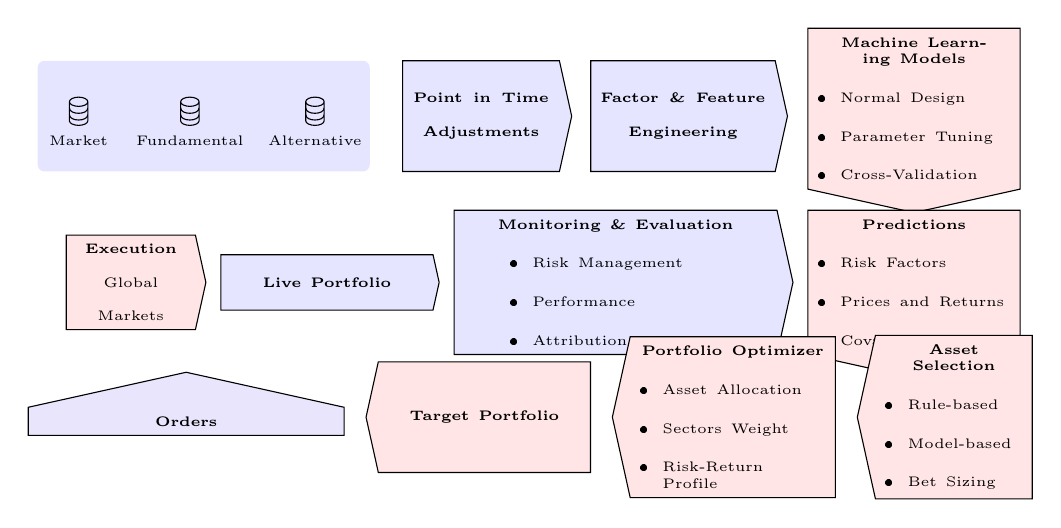
\begin{tikzpicture}
% data sources
\node[rectangle, rounded corners=0.25em,draw=none, minimum width=12em, minimum height=4em, fill=blue!10] (data_source) {};
\node[database, label={[label distance=0cm]180:\tiny{Market}}] (market) at ([xshift=1.5em] data_source.west) {};
\node[database, label={[label distance=0cm]180:\tiny{Fundamental}}] (fundamental) at ([xshift=-0.5em] data_source) {};
\node[database, label={[label distance=0cm]180:\tiny{Alternative}}] (alternative) at ([xshift=-2.0em] data_source.east) {};

\node[
    signal,signal to = east,
    fill=blue!10,draw=black,
    signal pointer angle=155,
    text width=5em,align=center,
    font=\color{black}\bfseries,
    minimum height=4em
    ] (pit_adj) at ([xshift=4.0em] data_source.east) {\tiny{Point in Time Adjustments}};
    
\node[
    signal,signal to = east,
    fill=blue!10,draw=black,
    signal pointer angle=155,
    text width=6em,align=center,
    font=\color{black}\bfseries,
    minimum height=4em
    ] (ffe) at ([xshift=4.0em] pit_adj.east) {\tiny{Factor \& Feature Engineering}};
    
\node[
    signal,signal to = south,
    signal pointer angle=155,
    fill=red!10,draw=black,
    text width=7em,align=center,
    font=\color{black},
    minimum height=2em
    ] (mml) at ([xshift=5.0em, yshift=-1.75em] ffe.north east) {
    \tiny{\textbf{Machine Learning Models}}
    \tiny{{\begin{itemize}[leftmargin=*]
        \item Normal Design
        \item Parameter Tuning
        \item Cross-Validation
    \end{itemize}}}};
    
\node[
    signal,signal to = south,
    signal pointer angle=155,
    fill=red!10,draw=black,
    text width=7em,align=center,
    font=\color{black},
    minimum height=2em
    ] (pred) at ([ yshift=-2.5em] mml.south) {
    \tiny{\textbf{Predictions}}
    \tiny{{\begin{itemize}[leftmargin=*]
        \item Risk Factors
        \item Prices and Returns
        \item Covariance
    \end{itemize}}}};

\node[
    signal,signal to = east,
    signal pointer angle=155,
    fill=blue!10,draw=black,
    text width=11em,align=center,
    font=\color{black},
    minimum height=2em,
    anchor=east
    ] (monitor_and_eval) at ([xshift=-0.5em] pred.west) {
    \tiny{\textbf{Monitoring \& Evaluation}}
    \tiny{{\begin{itemize}[]
        \item Risk Management
        \item Performance
        \item Attribution
    \end{itemize}}}};

\node[
    signal,signal to = east,
    signal pointer angle=155,
    fill=blue!10,draw=black,
    text width=7em,align=center,
    font=\color{black},
    minimum height=2em,
    anchor=east
    ] (live_portfolio) at ([xshift=-0.5em] monitor_and_eval.west) {
    \tiny{\textbf{Live Portfolio}}
    {\usebox{\lptable}}
    };
    
\node[
    signal,signal to = east,
    signal pointer angle=155,
    fill=red!10,draw=black,
    text width=4em,align=center,
    font=\color{black},
    minimum height=2em,
    anchor=east
    ] (execution) at ([xshift=-0.5em] live_portfolio.west) {
    \tiny{\textbf{Execution}}
    \tiny{Global Markets}
    };
    
\node[
    signal,signal to = north,
    signal pointer angle=155,
    fill=red!10!blue!10,draw=black,
    text width=10.75em,align=center,
    font=\color{black},
    minimum height=2em,
    anchor=north
    ] (orders) at ([xshift=2em, yshift=-1.5em] execution.south) {
    \tiny{\textbf{Orders}}
    \usebox{\orderstable}
    };
\node[
    signal,signal to = west,
    signal pointer angle=155,
    fill=red!10,draw=black,
    text width=7em,align=center,
    font=\color{black},
    minimum height=4em,
    anchor=west
    ] (target_portfolio) at ([xshift=0.75em, yshift=0.15em] orders.east) {
    \tiny{\textbf{Target Portfolio}}
    \usebox{\tptable}
    };
\node[
    signal,signal to = west,
    signal pointer angle=155,
    fill=red!10,draw=black,
    text width=6.75em,align=center,
    font=\color{black},
    minimum height=4em,
    anchor=west
    ] (portfolio_optimizer) at ([xshift=0.75em, yshift=-0em] target_portfolio.east) {
    \tiny{\textbf{Portfolio Optimizer}}
    \tiny{{\begin{itemize}[leftmargin=*]
        \item Asset Allocation
        \item Sectors Weight
        \item Risk-Return Profile
    \end{itemize}}}
    };
\node[
    signal,signal to = west,
    signal pointer angle=155,
    fill=red!10,draw=black,
    text width=5em,align=center,
    font=\color{black},
    minimum height=4em,
    anchor=west
    ] (asset_selection) at ([xshift=0.75em, yshift=-0em] portfolio_optimizer.east) {
    \tiny{\textbf{Asset Selection}}
    \tiny{{\begin{itemize}[leftmargin=*]
        \item Rule-based
        \item Model-based
        \item Bet Sizing
    \end{itemize}}}
    };
\end{tikzpicture}
\end{document}